%---------------------- begin chap 2 -------------
\cchapter{پیشینه و ادبیات پژوهش}
\label{chap:lit}
\pagebreak
\section{مقدمه}

لورم ایپسوم ( به انگلیسی \lr{lorem ipsum} ) متنی بی مفهوم است که تشکیل شده از کلمات معنی دار یا بی معنی کنار هم. کاربر با دیدن متن لورم ایپسوم تصور میکند متنی که در صفحه مشاهده میکند این متن واقعی و مربوط به توضیحات صفحه مورد نظر است واقعی است. حالا سوال اینجاست که این متن « لورم ایپسوم » به چه دردی میخورد و اساسا برای چه منظور و هدفی ساخته شده است؟ پیش از بوجود آمدن لورم ایپسوم ، طراحان وب سایت در پروژه های وب سایت و طراحان کرافیک در پروژه های طراحی کاتولوگ ، بروشور ، پوستر و ... همواره با این مشکل مواجه بودند که صفحات پروژه خود را پیش از آنکه متن اصلی توسط کارفرما ارائه گردد و در صفحه مورد نظر قرار گیرد چگونه پر کنند؟؟ اکثر طراحان با نوشتن یک جمله مانند «این یک متن نمونه است» ویا «توضیحات در این بخش قرار خواهند گرفت» و کپی آن به تعداد زیاد یک یا چند پاراگراف متن میساختند که تمامی متن ها و کلمات ، جملات و پاراگراف ها تکراری بود و از این رو منظره خوبی برای بیننده نداشت و ضمنا به هیچ وجه واقعی به نظر نمیرسید تا بتواند شکل و شمایل تمام شده پروژه را نشان دهد. از این رو متنی ساخته شد که با دو کلمه ( به فارسی : لورم ایپسوم ) آغاز میشد وبا همین نام در بین طراحان وب و گرافیک شناخته و به سرعت محبوب شد. وب سایت های سازنده لورم ایپسوم میتوانند هر تعداد کلمه و پاراگراف که بخواهید به صوورت تکراری یا غیر تکراری برایتان بسازند و تحویلتان بدهند تا از آنها در پروژه هایتان استفاده کنید. ( لورم ایپسوم فارسی) متن های لورم ایپسوم را به زبان فارسی و علاوه بر زبان فارسی به انگلیسی ، عربی ، ترکی استانبولی و ... برایتان میسازد. زبان های دیگر نیز رفته رفته به بانک اطلاعاتی لورم ایسپوم فارسی اضافه خواهند شد.  

\subsection{تاریخچه}

آغاز پژوهش در این زمینه را می‌توان به وِن\LTRfootnote{ Wen} و زیلین\LTRfootnote{ Xilin} \cite{Wu2005} 
در سال ۲۰۰۵ نسبت داد که الگوریتم ارایه‌شده‌ی پیشین خود را که برای تشخیص علایم حاوی متن در محیط به‌ کار گرفته‌ شده بود \cite{Chen2004}، به صور خاص بر روی ویدیوهای شهری اعمال کرد. این پژوهش از قید عمودی بودن صفحه‌ی تابلو استفاده نمود و متن درون تابلوها را با استفاده از یک روش افزایشی\LTRfootnote{ Incremental} تشخیص داد. پس از آن در سال ۲۰۰۶ توجه بیشتری به مساله‌ی تابلوهای راهنما شد \cite{reina2006adaptive, vazquez2006approach} و علاوه بر یک روش تطبیقی\LTRfootnote{ Adaptive} برای تقطیع، شناسایی متن با استفاده از ماشین بردار پشتیبان
\LTRfootnote{ Support Vector Machine (SVM)}
نیز در آن ارایه گردید. 


در این فصل در بخش \ref{sec:panelReview} به معرفی روش‌های به کار رفته در تشخیص تابلو می‌پردازیم و ایده‌های موجود در کارهای پیشین را بررسی می‌کنیم، سپس در بخش \ref{sec:textReview} به معرفی روش‌های تشخیص متن در تابلوی راهنما می‌پردازیم. در پایان هر بخش داده‌ها و نتایج به‌دست آمده را بررسی خواهیم کرد. 

\section{تشخیص تابلوهای راهنما}
\label{sec:panelReview}

در این بخش به بررسی روش‌های موجود برای تشخیص تابلوهای راهنما پرداخته‌ایم و ایده‌های به کاررفته شده در پژوهش‌های موجود گردآوری و بررسی شده‌اند. در تشخیص تابلوی راهنما، مکان‌یابی تابلو و رفع افکنش\LTRfootnote{ Perspective} آن از اهمیت ویژه‌ای برخوردار است. قیود فیزیکی مانند مسطح بودن صفحه‌ی تابلو و یا مکان قرارگیری آن در جاده، و ویژگی‌های ظاهری مانند شکل و رنگ از جمله قیود به کار رفته در پژوهش‌های موجود هستند که در ادامه به بررسی آن‌ها در پژوهش‌های انجام‌شده می‌پردازیم. 

%---------------------- روش اول -------------
\subsection{عمودی بودن صفحه‌ی تابلوی راهنما}

در روش زیلین \cite{Wu2005}، تابلوهای راهنما طی دو مرحله استخراج می‌شوند. 

%---------------------- روش اول - ۱  -------------


\subsubsection{خوشه‌بندی نقاط با تحلیل رنگ}
ابتدا نقاط قابل تمییز\LTRfootnote{ Discriminative points } با روش شی-توماسی\LTRfootnote{ Shi-Tomasi} \cite{shi1994good}، استخراج می‌شوند. نقاطی که توسط این روش استخراج می‌شوند نقاطی خوب هستند و به آسانی تعقیب می‌شوند. در این روش ماتریس لاپلاسی برای هر نقطه در تصویر محاسبه می‌شود و مقدار ویژه‌ی کمینه‌ی $\lambda_m$ برای آن یافت می‌شود. در کل تصویر، بیشینه‌ی $\lambda_m$ یافت می‌شود و $\lambda_{max}$ نامیده می‌شود. نقاطی از تصویر که $\lambda_m$ آن‌ها بیش از 
$\% 10$ 
مقدار $\lambda_{max}$ باشد نگاه داشته می‌شوند. از این مجموعه نقاط، نقاطی که در همسایگی
 $ 3 \times 3 $ 

..........
توزیع رنگ نقاط در همسایگی هر نقطه‌ی ویژگی توسط مدل ترکیبی گاوسی\LTRfootnote{ Gaussian Mixture Model (GMM)} مدل می‌شود:
\begin{equation}
g(c) = \beta G_f(\mu_f , \theta_f) + (1 - \beta)G_b(\mu_b , \theta_b), \quad 0 \le \beta \le 1
\label{eq:GMM}
\end{equation}
که در آن $G_f$ و $G_b$ به ترتیب توزیع رنگ پیش‌زمینه و پس‌زمینه هستند. به‌این ترتیب، هر نقطه‌ی ویژگی می‌تواند با یک بردار 
$(\beta , \mu_f , \mu_b , \theta_f , \theta_b)$
که پارامترهای مدل ترکیبی گاوسی در آن نقطه‌ است نشان داده شود. وقتی اشباع رنگ\LTRfootnote{ Saturation} کم نباشد فضای رنگی اچ‌اس‌آی به دلیل مقاوت بیشتر در برابر تغییرات نوری انتخاب مناسب‌تری است که در پژوهش‌ یاد شده، مولفه‌ی اِچ آن به کار گرفته شده‌ است. با استفاده از پارامترهای مدل ترکیبی گاوسی در هر نقطه و با استفاده از روش کا-میانگین\LTRfootnote{ K-means} خوشه‌بندی انجام می‌شود و خوشه‌های
$\lbrace C_1^t , C_2^t , \dots , C_K^t \rbrace$
در زمان $t$ به‌دست می‌آیند که در پژوهش یادشده، $K$ برابر مقدار ثابت ۱۰ انتخاب شده‌است و نشان‌دهنده‌ی تعداد خوشه‌هاست. به این ترتیب، نقاطی که توزیع رنگ پس‌زمینه و پیش‌زمینه‌ی مشابه دارند در یک خوشه قرار می‌گیرند. 
$C_i^t = \left[ \ p_j^t , \dots , p_k^t \ \right] $
یک خوشه از نقطه‌ی ویژگی $j$م تا نقطه‌ی ویژگی $k$م معرفی شده‌است. پس از محاسبه‌ی یک مستطیل محدود‌کننده‌ی کمینه\LTRfootnote{ Minimu-Bounding Rectangle (MBR)}، تابلوهای راهنما در این نواحی مکان‌یابی می‌شوند. 


%---------------------- روش اول - ۲ -------------


\subsubsection{فرض عمودی بودن صفحه}

با در نظر گرفتن دو فرض زیر، با استفاده از سه نقطه یا بیشتر در دو فریم متوالی جهت تابلوی راهنما استخراج شده‌است: 
\begin{enumerate}
\item متن مورد نظر روی یک صفحه‌ی مسطح و عمودی است.
\item محور چشمی دوربین افقی می‌باشد و حرکت دوربین نیز در راستای همین محور است.
\end{enumerate}
با در نظر گرفتن سه محور مختصات برای فریم اول، فریم دوم و دوربین، و مدل کردن دوربین به صورت نقطه‌ای، اطلاعاتی در مورد صلب بودن صفحه‌ی یافت شده و عمودی بودن آن به دست می‌آید. با توجه به شکل \ref{fig:p1-worlds}، برای سه نقطه‌ی $P_2$، $P_1$ و $P_3$ در دو فریم متوالی $t_0$ و $t_1$ خواهیم داشت: 
\begin{equation}
{\left( \begin{array}{c}
x_i^{t_0} \\
y_i^{t_0} \end{array} \right) } = {f \over Z_i}
{
\left( \begin{array}{c}
X_i \\
Y_i \end{array} \right) } \quad , \quad 
{\left( \begin{array}{c}
x_i^{t_1} \\
y_i^{t_1} \end{array} \right) } = {{f} \over {Z_i - d }}
{
\left( \begin{array}{c}
X_i \\
Y_i \end{array} \right) } \quad , \ i = 1, 2, 3.
\end{equation}
که در آن $f$ فاصله کانونی دوربین است و حروف بزرگ در دستگاه مختصات دوربین و حروف کوچک در دستگاه مختصات تصویر هستند و $d$ جابه‌جایی خودرو بین دو فریم متوالی است که در عمل مقدار کوچکی است.
\begin{figure}[t]
\centering
    	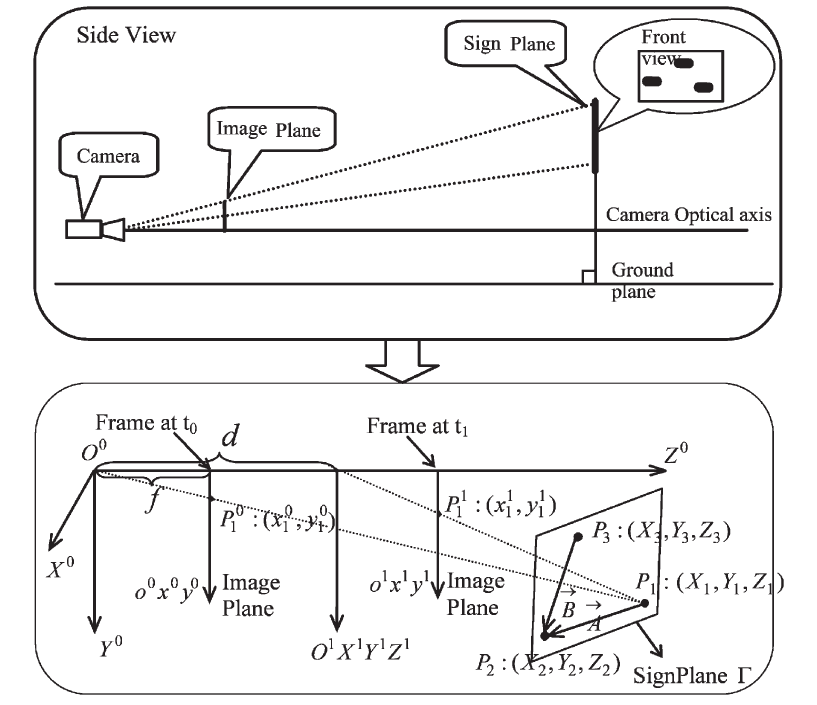
\includegraphics[width=13cm]{Figures/p1-worlds.png}
\caption[دستگاه‌های مختصات]{دستگاه‌های مختصات در نظر گرفته شده \cite{Wu2005}}
\label{fig:p1-worlds}
\end{figure}
در این پژوهش برای ارزیابی روش تشخیص، از ۲۲ ویدیوی ۳۰ ثانیه‌ای استفاده شده‌است که از روی یک خودروی در حال حرکت با سرعت‌ها و شرایط نوری متفاوت تهیه شده‌است و در مجموع دارای ۹۲ تابلوی راهنما می‌باشد. تشخیص درست 
$\% 92.4$ 
و نرخ اعلام‌های غلط 
$\% 17.7$
اعلام شده‌است. معیار درستی تشخیص همپوشانی بیش از $\% 80$ مساحت مستطیل تشخیص‌ داده‌شده و داده‌ی حقیقی زمینه‌\LTRfootnote{ Ground truth data} است. داده‌های حقیقی زمینه ابتدا توسط خود سیستم تولید شده‌اند و سپس توسط انسان به صورت دستی اصلاح شده‌اند. این داده‌ها برای تست و بررسی در دسترس نیستند.
%---------------------- روش دوم -------------
\subsection{تحلیل شکل و بازیابی جهت}

لورم ایپسوم ( به انگلیسی \lr{lorem ipsum} ) متنی بی مفهوم است که تشکیل شده از کلمات معنی دار یا بی معنی کنار هم. کاربر با دیدن متن لورم ایپسوم تصور میکند متنی که در صفحه مشاهده میکند این متن واقعی و مربوط به توضیحات صفحه مورد نظر است واقعی است. حالا سوال اینجاست که این متن « لورم ایپسوم » به چه دردی میخورد و اساسا برای چه منظور و هدفی ساخته شده است؟ پیش از بوجود آمدن لورم ایپسوم ، طراحان وب سایت در پروژه های وب سایت و طراحان کرافیک در پروژه های طراحی کاتولوگ ، بروشور ، پوستر و ... همواره با این مشکل مواجه بودند که صفحات پروژه خود را پیش از آنکه متن اصلی توسط کارفرما ارائه گردد و در صفحه مورد نظر قرار گیرد چگونه پر کنند؟؟ اکثر طراحان با نوشتن یک جمله مانند «این یک متن نمونه است» ویا «توضیحات در این بخش قرار خواهند گرفت» و کپی آن به تعداد زیاد یک یا چند پاراگراف متن میساختند که تمامی متن ها و کلمات ، جملات و پاراگراف ها تکراری بود و از این رو منظره خوبی برای بیننده نداشت و ضمنا به هیچ وجه واقعی به نظر نمیرسید تا بتواند شکل و شمایل تمام شده پروژه را نشان دهد. از این رو متنی ساخته شد که با دو کلمه ( به فارسی : لورم ایپسوم ) آغاز میشد وبا همین نام در بین طراحان وب و گرافیک شناخته و به سرعت محبوب شد. وب سایت های سازنده لورم ایپسوم میتوانند هر تعداد کلمه و پاراگراف که بخواهید به صوورت تکراری یا غیر تکراری برایتان بسازند و تحویلتان بدهند تا از آنها در پروژه هایتان استفاده کنید. ( لورم ایپسوم فارسی) متن های لورم ایپسوم را به زبان فارسی و علاوه بر زبان فارسی به انگلیسی ، عربی ، ترکی استانبولی و ... برایتان میسازد. زبان های دیگر نیز رفته رفته به بانک اطلاعاتی لورم ایسپوم فارسی اضافه خواهند شد.  
می‌کنند. 
\begin{figure}[t]
\centering
    	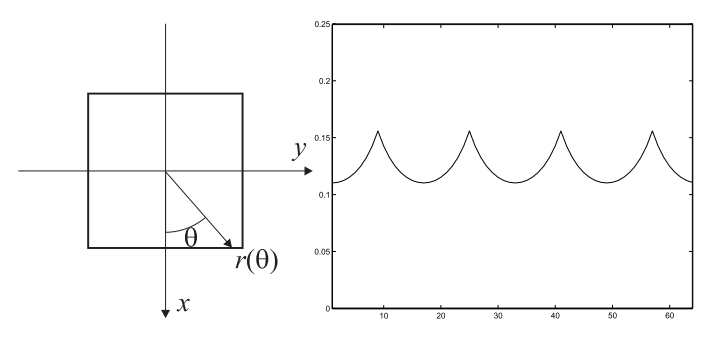
\includegraphics[width=10cm]{Figures/fft.png}
\caption[اثر (شعاعی) مستطیل]{اثر (شعاعی) مستطیل \cite{reina2006adaptive}}
\label{fig:fft}
\end{figure}
در این پژوهش، از ۶۴ نقطه روی هر لکه استفاده شده‌است که از ۰ تا $2\pi$ رادیان برای تولید اثر، شرکت داده شده‌اند. سپس مقادیر حاصل از اعمال تبدیل فوریه‌ی سریع بر روی اثر لکه با مقادیر حاصل از اعمال تبدیل فوریه‌ی سریع بر روی شکل مستطیل ایده‌آل مقایسه می‌شوند و اشکال مستطیلی به عنوان تابلو انتخاب می‌شوند. مزیت این روش مقایسه در آن است که اعمال تبدیل فوریه روی اثر شعاعی نسبت به چرخش و تغییر شکل‌های جزیی ناشی از تصویربرداری و تغییر زاویه‌ی دید مقاوم است. 
لورم ایپسوم ( به انگلیسی \lr{lorem ipsum} ) متنی بی مفهوم است که تشکیل شده از کلمات معنی دار یا بی معنی کنار هم. کاربر با دیدن متن لورم ایپسوم تصور میکند متنی که در صفحه مشاهده میکند این متن واقعی و مربوط به توضیحات صفحه مورد نظر است واقعی است. حالا سوال اینجاست که این متن « لورم ایپسوم » به چه دردی میخورد و اساسا برای چه منظور و هدفی ساخته شده است؟ پیش از بوجود آمدن لورم ایپسوم ، طراحان وب سایت در پروژه های وب سایت و طراحان کرافیک در پروژه های طراحی کاتولوگ ، بروشور ، پوستر و ... همواره با این مشکل مواجه بودند که صفحات پروژه خود را پیش از آنکه متن اصلی توسط کارفرما ارائه گردد و در صفحه مورد نظر قرار گیرد چگونه پر کنند؟؟ اکثر طراحان با نوشتن یک جمله مانند «این یک متن نمونه است» ویا «توضیحات در این بخش قرار خواهند گرفت» و کپی آن به تعداد زیاد یک یا چند پاراگراف متن میساختند که تمامی متن ها و کلمات ، جملات و پاراگراف ها تکراری بود و از این رو منظره خوبی برای بیننده نداشت و ضمنا به هیچ وجه واقعی به نظر نمیرسید تا بتواند شکل و شمایل تمام شده پروژه را نشان دهد. از این رو متنی ساخته شد که با دو کلمه ( به فارسی : لورم ایپسوم ) آغاز میشد وبا همین نام در بین طراحان وب و گرافیک شناخته و به سرعت محبوب شد. وب سایت های سازنده لورم ایپسوم میتوانند هر تعداد کلمه و پاراگراف که بخواهید به صوورت تکراری یا غیر تکراری برایتان بسازند و تحویلتان بدهند تا از آنها در پروژه هایتان استفاده کنید. ( لورم ایپسوم فارسی) متن های لورم ایپسوم را به زبان فارسی و علاوه بر زبان فارسی به انگلیسی ، عربی ، ترکی استانبولی و ... برایتان میسازد. زبان های دیگر نیز رفته رفته به بانک اطلاعاتی لورم ایسپوم فارسی اضافه خواهند شد.  
لورم ایپسوم ( به انگلیسی \lr{lorem ipsum} ) متنی بی مفهوم است که تشکیل شده از کلمات معنی دار یا بی معنی کنار هم. کاربر با دیدن متن لورم ایپسوم تصور میکند متنی که در صفحه مشاهده میکند این متن واقعی و مربوط به توضیحات صفحه مورد نظر است واقعی است. حالا سوال اینجاست که این متن « لورم ایپسوم » به چه دردی میخورد و اساسا برای چه منظور و هدفی ساخته شده است؟ پیش از بوجود آمدن لورم ایپسوم ، طراحان وب سایت در پروژه های وب سایت و طراحان کرافیک در پروژه های طراحی کاتولوگ ، بروشور ، پوستر و ... همواره با این مشکل مواجه بودند که صفحات پروژه خود را پیش از آنکه متن اصلی توسط کارفرما ارائه گردد و در صفحه مورد نظر قرار گیرد چگونه پر کنند؟؟ اکثر طراحان با نوشتن یک جمله مانند «این یک متن نمونه است» ویا «توضیحات در این بخش قرار خواهند گرفت» و کپی آن به تعداد زیاد یک یا چند پاراگراف متن میساختند که تمامی متن ها و کلمات ، جملات و پاراگراف ها تکراری بود و از این رو منظره خوبی برای بیننده نداشت و ضمنا به هیچ وجه واقعی به نظر نمیرسید تا بتواند شکل و شمایل تمام شده پروژه را نشان دهد. از این رو متنی ساخته شد که با دو کلمه ( به فارسی : لورم ایپسوم ) آغاز میشد وبا همین نام در بین طراحان وب و گرافیک شناخته و به سرعت محبوب شد. وب سایت های سازنده لورم ایپسوم میتوانند هر تعداد کلمه و پاراگراف که بخواهید به صوورت تکراری یا غیر تکراری برایتان بسازند و تحویلتان بدهند تا از آنها در پروژه هایتان استفاده کنید. ( لورم ایپسوم فارسی) متن های لورم ایپسوم را به زبان فارسی و علاوه بر زبان فارسی به انگلیسی ، عربی ، ترکی استانبولی و ... برایتان میسازد. زبان های دیگر نیز رفته رفته به بانک اطلاعاتی لورم ایسپوم فارسی اضافه خواهند شد.  

\begin{figure}[!htb]
\centering
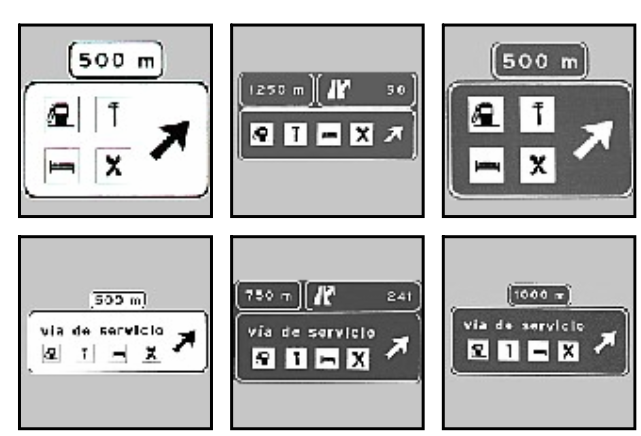
\includegraphics[width=11cm]{Figures/adaptive-types.png}
\caption[تابلوهای معرفی شده]{تابلوهای معرفی شده \cite{vazquez2006approach}.
به ترتیب از چپ به راست و از بالا به پایین:
 \lr{S-266a S-266, S-264, S-263a, S-263, S-261}
}
\label{fig:adaptive-types}
\end{figure}

\begin{table}[!htb]
\begin{center}
\def\arraystretch{2.5}
\begin{tabular}{|c|c|c|c|c|c|c|}
\hline
نوع دسته & 
\lr{S-266a} & \lr{S-266}  & \lr{S-264} & \lr{S-263a} & \lr{S-263} & \lr{S-261}\\
\hline
دقت تشخیص & 
$\% 83.19 $ & $\% 77.78 $ & $\% 75.00 $  & $\% 86.67 $ & $\% 82.35 $ & $\% 78.00$ \\
\hline
دقت دسته‌بندی & 
$\% 83.19 $ & $\% 77.78 $ & $\% 75.00 $  & $\% 86.67$ & $ \%82.35 $ & $\% 78.00 $ \\
\hline
\end{tabular}
\caption[درصد تشخیص درست]{درصد تشخیص درست دسته‌های معرفی شده \cite{vazquez2006approach}}
\label{tab:adaptive}
\end{center}
\end{table}
لورم ایپسوم ( به انگلیسی \lr{lorem ipsum} ) متنی بی مفهوم است که تشکیل شده از کلمات معنی دار یا بی معنی کنار هم. کاربر با دیدن متن لورم ایپسوم تصور میکند متنی که در صفحه مشاهده میکند این متن واقعی و مربوط به توضیحات صفحه مورد نظر است واقعی است. حالا سوال اینجاست که این متن « لورم ایپسوم » به چه دردی میخورد و اساسا برای چه منظور و هدفی ساخته شده است؟ پیش از بوجود آمدن لورم ایپسوم ، طراحان وب سایت در پروژه های وب سایت و طراحان کرافیک در پروژه های طراحی کاتولوگ ، بروشور ، پوستر و ... همواره با این مشکل مواجه بودند که صفحات پروژه خود را پیش از آنکه متن اصلی توسط کارفرما ارائه گردد و در صفحه مورد نظر قرار گیرد چگونه پر کنند؟؟ اکثر طراحان با نوشتن یک جمله مانند «این یک متن نمونه است» ویا «توضیحات در این بخش قرار خواهند گرفت» و کپی آن به تعداد زیاد یک یا چند پاراگراف متن میساختند که تمامی متن ها و کلمات ، جملات و پاراگراف ها تکراری بود و از این رو منظره خوبی برای بیننده نداشت و ضمنا به هیچ وجه واقعی به نظر نمیرسید تا بتواند شکل و شمایل تمام شده پروژه را نشان دهد. از این رو متنی ساخته شد که با دو کلمه ( به فارسی : لورم ایپسوم ) آغاز میشد وبا همین نام در بین طراحان وب و گرافیک شناخته و به سرعت محبوب شد. وب سایت های سازنده لورم ایپسوم میتوانند هر تعداد کلمه و پاراگراف که بخواهید به صوورت تکراری یا غیر تکراری برایتان بسازند و تحویلتان بدهند تا از آنها در پروژه هایتان استفاده کنید. ( لورم ایپسوم فارسی) متن های لورم ایپسوم را به زبان فارسی و علاوه بر زبان فارسی به انگلیسی ، عربی ، ترکی استانبولی و ... برایتان میسازد. زبان های دیگر نیز رفته رفته به بانک اطلاعاتی لورم ایسپوم فارسی اضافه خواهند شد.  
%---------------------- روش سوم -------------
\subsection{استفاده از ویژگی‌های ظاهری و مدل کیسه کلمات بینایی}
\label{subsec:gonzalez}

 از یک لبه‌یاب کنی اصلاح شده استفاده شده‌است. دو اصلاح انجام شده بر روی این لبه‌یاب، یکی استفاده از هسته‌ی زیر برای افزایش تضاد لبه‌ها است: 
\begin{equation}
\begin{bmatrix} 0 & -1 & 0 \\ -1 & 5 & -1 \\ 0 & -1 & 0 \end{bmatrix}
\end{equation}

زاویه‌ی چرخش 
$\alpha$
 تابلو در نظر گرفته می‌شود. به این ترتیب یک ماتریس چرخش براتبدیل نقاط $x$ و $y$ تابلو ساخته می‌شود:
 
\begin{equation}
\begin{bmatrix} \cos \alpha & \sin \alpha & (1-\cos \alpha) x_0 - \sin \alpha \cdot y_0 \\
-\sin \alpha & \cos \alpha &  \sin \alpha \cdot x_0 + (1-\cos \alpha) y_0
\end{bmatrix}
\end{equation}
برای تشخیص نواحی آبی‌رنگ، از \lr{AND} منطقی سه روش زیر استفاده شده‌است: 
\begin{itemize}
\item{آستانه‌ی رنگ قرمز}:
مقدار مولفه‌ی آر در فضای آرجی‌بی کمتر از حد آستانه‌ای ۹۰ باشد.
\item{آستانه‌ی رنگ آبی}:
محدوده‌ی مولفه‌ی اچ در فضای اچ‌اس‌وی\LTRfootnote{ HSV} بین مقادیر آستانه‌ای ۲۰۰ و ۲۸۰ درجه باشد. 
\item{روش اوتسو\LTRfootnote{ Otsu} \cite{otsu1975threshold} بر روی تفاضل مولفه‌ی قرمز و آبی}:
در این روش تصویر حاصل از قدر مطلق تفاضل مولفه‌ی قرمز و آبی به الگوریتم اوتسو داده‌ شده‌است. این الگوریتم برای دودویی کردن تصاویر به کار می‌رود، به شکلی که حد آستانه‌ی مناسبی برای آستانه‌ای کردن تصویر می‌یابد که در آن آستانه، واریانس درون دو دسته‌ی ایجاد شده (برای مثال، پس‌زمینه و پیش‌زمینه) کمینه باشد.
\end{itemize}
برای تشخیص نواحی سفیدرنگ، از روش نواحی حدی بیشینه پایدار استفاده شده‌است که به کمک آن می‌توان نواحی روشن روی نواحی تیره را تشخیص داد و پیشتر توضیح داده‌شد. 

در شکل‌های \ref{fig:bluep5} و \ref{fig:withep5} نتایج این دو آستانه‌ای کردن را مشاهده می‌کنید.
\begin{figure}[h]
\centering
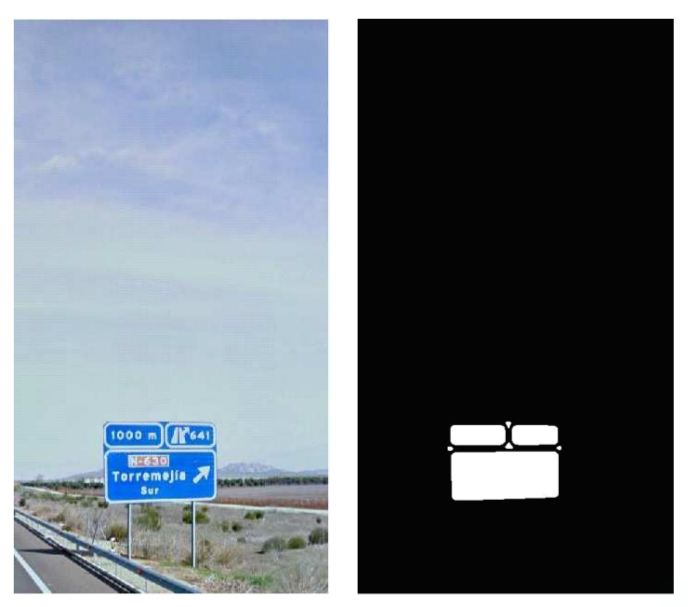
\includegraphics[width=7cm]{Figures/bluepp5.png}
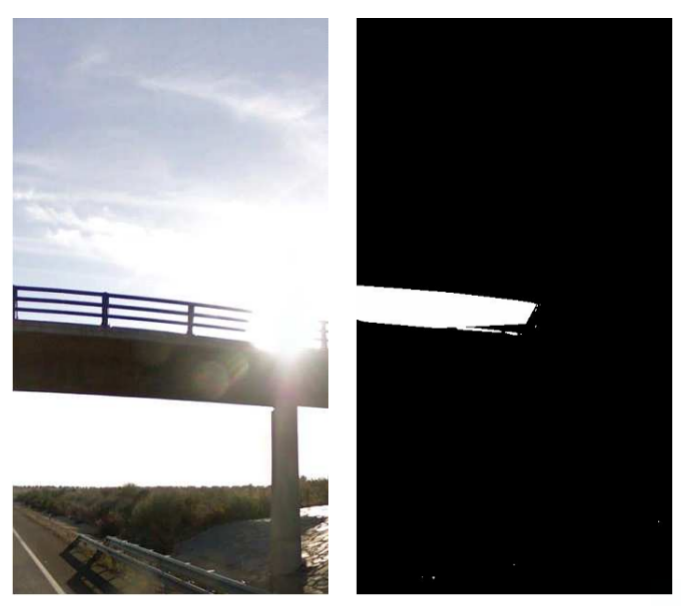
\includegraphics[width=7cm]{Figures/blue-fp5.png}
\caption[آستانه‌ای سازی رنگ آبی]{آستانه‌ای سازی رنگ آبی \cite{gonzalez2013traffic} (راست نمونه‌ی مثبت و چپ نمونه‌ی منفی)}
\label{fig:bluep5}
\end{figure}
\begin{figure}[h]
\centering
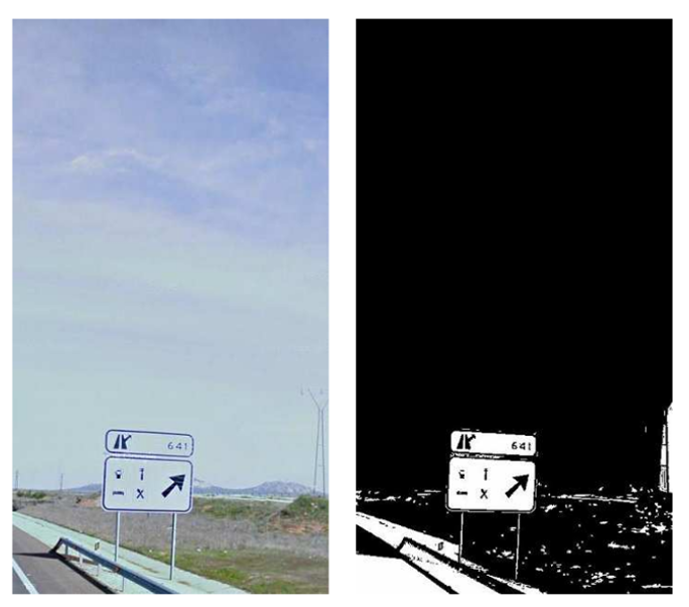
\includegraphics[width=7cm]{Figures/withe-pp5.png}
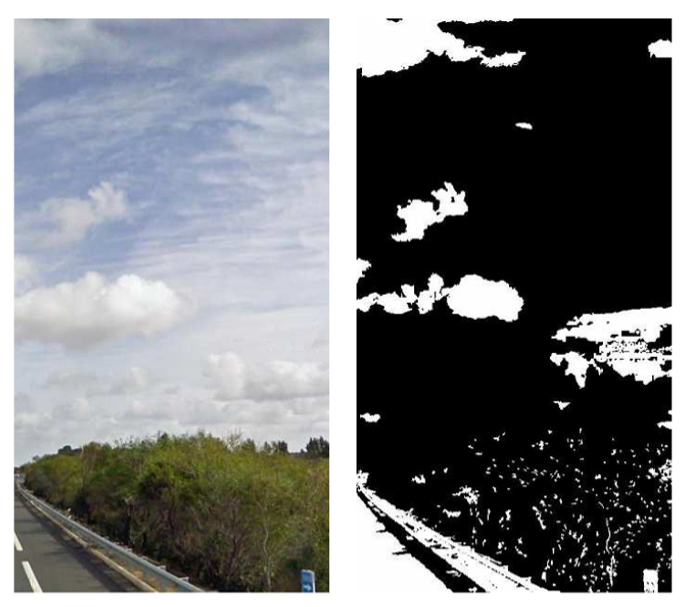
\includegraphics[width=7cm]{Figures/withe-fp5.png}
\caption[آستانه‌ای سازی رنگ سفید]{آستانه‌ای سازی رنگ سفید \cite{gonzalez2013traffic} (راست نمونه‌ی مثبت و چپ نمونه‌ی منفی)}
\label{fig:withep5}
\end{figure}

 بهترین نتایج با توصیف‌گر هیستوگرام دگرگون‌شده‌ی رنگ در جدول \ref{tab:tch} آورده شده‌است. 
\begin{table}[h]
\begin{center}
\def\arraystretch{2}
\begin{tabular}{|c|c|c|c|c|}
\hline
نوع دسته & 
نرخ تشخیص & حساسیت & تشخیص & معیار اِف \\
\hline

بالای جاده & 
$\% 98.70$ & $0.8821$ & $0.8817$ & $0.8819$ \\
\hline

کنار جاده & 
$\% 98.15$ & $0.7464$ & $0.4772$ & $0.6118$ \\
\hline
\end{tabular}
\caption[ارزیابی با توصیف‌گر هیستوگرام دگرگون‌شده‌ی رنگ]{ارزیابی با توصیف‌گر هیستوگرام دگرگون‌شده‌ی رنگ \cite{gonzalez2013traffic}}
\label{tab:tch}
\end{center}
\end{table}
%-----------------‌----- روش چهارم -------------
\subsection{اطلاعات ساختاری و زمانی}

دقت\LTRfootnote{ Precision}، یادآوری\LTRfootnote{ Recall} و معیار اِف به ترتیب در فرمول‌های \eqref{eq:precision}، \eqref{eq:recall} و \eqref{eq:fmeasure} آورده شده‌اند.
\begin{equation}
{\text{دقت}}  = { {TP} \over {TP + FP}}
\label{eq:precision}
\end{equation}
\begin{equation}
{\text{یادآوری}}  = { {TP} \over {TP + FN}}
\label{eq:recall}
\end{equation}
\begin{equation}
{\text{معیار اِف}}  = 2 * { {\text{دقت}*\text{یادآوری}} \over {\text{دقت}+\text{یادآوری}}}
\label{eq:fmeasure}
\end{equation}
 ارزیابی این پژوهش روی این پایگاه داده در مقایسه با روش‌های دیگر در جدول \ref{tab:mirmehdi} آورده شده‌است. 
\begin{table}[h]
\begin{center}
\def\arraystretch{2}
\begin{tabular}{|c|c|c|c|c|}
\hline
پژوهش & 
دقت & یادآوری & معیار اِف \\
\hline

رینا و همکاران \cite{reina2006adaptive} & 
$0.58$ & $0.64$ & $0.61$  \\
\hline

گنزالز و همکاران \cite{gonzalez2012text} & 
$0.54$ & $0.68$ & $0.60$  \\
\hline
میرمهدی و همکاران \cite{Greenhalgh2015} & 
$0.96$ & $0.90$ & $0.93$  \\
\hline
\end{tabular}
\caption[ارزیابی انجام‌شده در روش گنزالز]{ارزیابی انجام‌شده در\cite{gonzalez2013traffic}}
\label{tab:mirmehdi}
\end{center}
\end{table}
%-----------------‌----- پایان تشخیص تابلو -------------
\section{تشخیص متن در تابلوی راهنما}
\label{sec:textReview}
پس از استخراج تابلوهای راهنما، جست‌وجو به دنبال متن درون آن آغاز می‌گردد.
\subsection{روش‌های مبتنی بر لبه}

لورم ایپسوم ( به انگلیسی \lr{lorem ipsum} ) متنی بی مفهوم است که تشکیل شده از کلمات معنی دار یا بی معنی کنار هم. کاربر با دیدن متن لورم ایپسوم تصور میکند متنی که در صفحه مشاهده میکند این متن واقعی و مربوط به توضیحات صفحه مورد نظر است واقعی است. حالا سوال اینجاست که این متن « لورم ایپسوم » به چه دردی میخورد و اساسا برای چه منظور و هدفی ساخته شده است؟ پیش از بوجود آمدن لورم ایپسوم ، طراحان وب سایت در پروژه های وب سایت و طراحان کرافیک در پروژه های طراحی کاتولوگ ، بروشور ، پوستر و ... همواره با این مشکل مواجه بودند که صفحات پروژه خود را پیش از آنکه متن اصلی توسط کارفرما ارائه گردد و در صفحه مورد نظر قرار گیرد چگونه پر کنند؟؟ اکثر طراحان با نوشتن یک جمله مانند «این یک متن نمونه است» ویا «توضیحات در این بخش قرار خواهند گرفت» و کپی آن به تعداد زیاد یک یا چند پاراگراف متن میساختند که تمامی متن ها و کلمات ، جملات و پاراگراف ها تکراری بود و از این رو منظره خوبی برای بیننده نداشت و ضمنا به هیچ وجه واقعی به نظر نمیرسید تا بتواند شکل و شمایل تمام شده پروژه را نشان دهد. از این رو متنی ساخته شد که با دو کلمه ( به فارسی : لورم ایپسوم ) آغاز میشد وبا همین نام در بین طراحان وب و گرافیک شناخته و به سرعت محبوب شد. وب سایت های سازنده لورم ایپسوم میتوانند هر تعداد کلمه و پاراگراف که بخواهید به صوورت تکراری یا غیر تکراری برایتان بسازند و تحویلتان بدهند تا از آنها در پروژه هایتان استفاده کنید. ( لورم ایپسوم فارسی) متن های لورم ایپسوم را به زبان فارسی و علاوه بر زبان فارسی به انگلیسی ، عربی ، ترکی استانبولی و ... برایتان میسازد. زبان های دیگر نیز رفته رفته به بانک اطلاعاتی لورم ایسپوم فارسی اضافه خواهند شد.  
%-------------- رنگ
%---------------- چینش متن

\subsection{تقطیع تطبیقی}
لورم ایپسوم ( به انگلیسی \lr{lorem ipsum} ) متنی بی مفهوم است که تشکیل شده از کلمات معنی دار یا بی معنی کنار هم. کاربر با دیدن متن لورم ایپسوم تصور میکند متنی که در صفحه مشاهده میکند این متن واقعی و مربوط به توضیحات صفحه مورد نظر است واقعی است. حالا سوال اینجاست که این متن « لورم ایپسوم » به چه دردی میخورد و اساسا برای چه منظور و هدفی ساخته شده است؟ پیش از بوجود آمدن لورم ایپسوم ، طراحان وب سایت در پروژه های وب سایت و طراحان کرافیک در پروژه های طراحی کاتولوگ ، بروشور ، پوستر و ... همواره با این مشکل مواجه بودند که صفحات پروژه خود را پیش از آنکه متن اصلی توسط کارفرما ارائه گردد و در صفحه مورد نظر قرار گیرد چگونه پر کنند؟؟ اکثر طراحان با نوشتن یک جمله مانند «این یک متن نمونه است» ویا «توضیحات در این بخش قرار خواهند گرفت» و کپی آن به تعداد زیاد یک یا چند پاراگراف متن میساختند که تمامی متن ها و کلمات ، جملات و پاراگراف ها تکراری بود و از این رو منظره خوبی برای بیننده نداشت و ضمنا به هیچ وجه واقعی به نظر نمیرسید تا بتواند شکل و شمایل تمام شده پروژه را نشان دهد. از این رو متنی ساخته شد که با دو کلمه ( به فارسی : لورم ایپسوم ) آغاز میشد وبا همین نام در بین طراحان وب و گرافیک شناخته و به سرعت محبوب شد. وب سایت های سازنده لورم ایپسوم میتوانند هر تعداد کلمه و پاراگراف که بخواهید به صوورت تکراری یا غیر تکراری برایتان بسازند و تحویلتان بدهند تا از آنها در پروژه هایتان استفاده کنید. ( لورم ایپسوم فارسی) متن های لورم ایپسوم را به زبان فارسی و علاوه بر زبان فارسی به انگلیسی ، عربی ، ترکی استانبولی و ... برایتان میسازد. زبان های دیگر نیز رفته رفته به بانک اطلاعاتی لورم ایسپوم فارسی اضافه خواهند شد.  

 
\begin{table}[h]
\begin{center}
\def\arraystretch{2}
\begin{tabular}{|c|c|c|c|c|c|}
\hline
 خطوط متن (\lr{T}) & خطوط متن (\lr{F}) & اجزا (\lr{T}) & اجزا (\lr{F}) & کلمات (\lr{T}) & کلمات (\lr{F}) \\
\hline
 $98.56$ & $0.56$ & $96.64$ & $1.72$ & $84.35$ & $3.15$ \\
\hline
\end{tabular}
\caption[نرخ تشخیص روش گنزالز]{درصد نرخ تشخیص روش گنزالز \cite{Gonzalez2009}}
\label{tab:n1text}
\end{center}
\end{table}
\begin{center}
\begin{figure}[h]
\centering
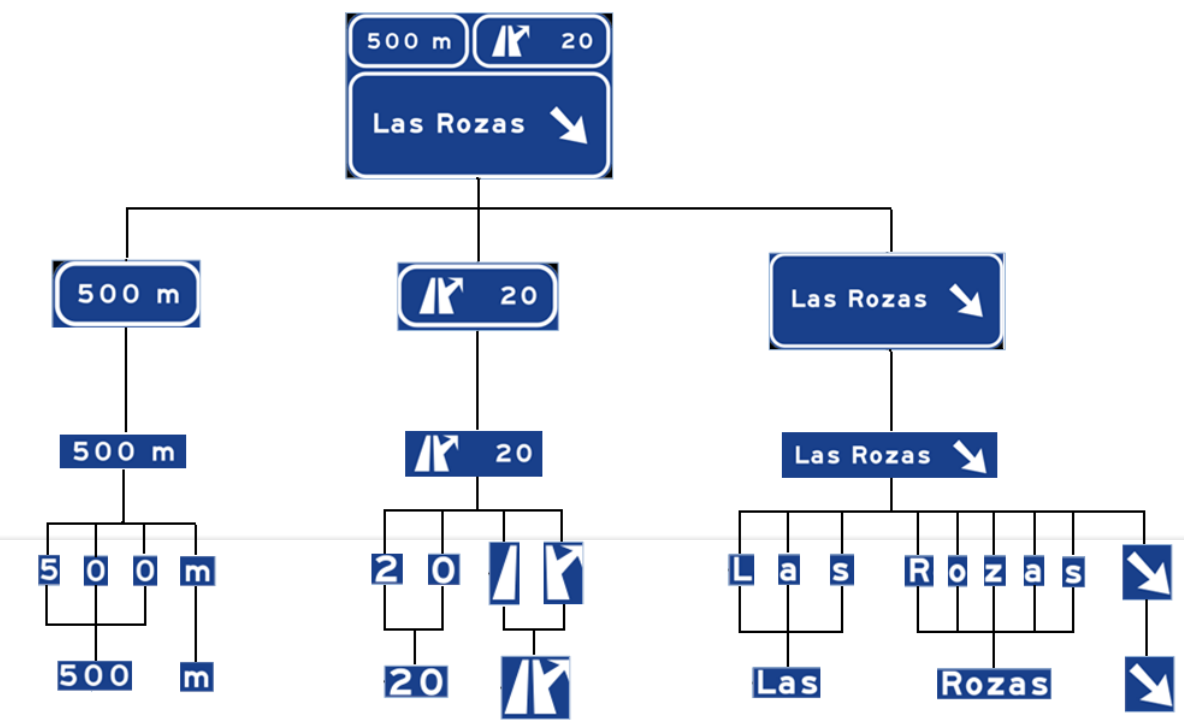
\includegraphics[width=14cm]{n1hir.png}
\caption[سلسله‌مراتب در روش گنزالز]{سلسله‌مراتب در روش گنزالز \cite{Gonzalez2009}. به ترتیب از بالا به پایین: تابلو، قاب‌های اطلاعاتی، خطوط، اجزا و حروف، کلمات.}
\label{fig:n1hir}
\end{figure}
\end{center}

\subsection{اجزای متصل و نواحی حدی بیشینه پایدار}
لورم ایپسوم ( به انگلیسی \lr{lorem ipsum} ) متنی بی مفهوم است که تشکیل شده از کلمات معنی دار یا بی معنی کنار هم. کاربر با دیدن متن لورم ایپسوم تصور میکند متنی که در صفحه مشاهده میکند این متن واقعی و مربوط به توضیحات صفحه مورد نظر است واقعی است. حالا سوال اینجاست که این متن « لورم ایپسوم » به چه دردی میخورد و اساسا برای چه منظور و هدفی ساخته شده است؟ پیش از بوجود آمدن لورم ایپسوم ، طراحان وب سایت در پروژه های وب سایت و طراحان کرافیک در پروژه های طراحی کاتولوگ ، بروشور ، پوستر و ... همواره با این مشکل مواجه بودند که صفحات پروژه خود را پیش از آنکه متن اصلی توسط کارفرما ارائه گردد و در صفحه مورد نظر قرار گیرد چگونه پر کنند؟؟ اکثر طراحان با نوشتن یک جمله مانند «این یک متن نمونه است» ویا «توضیحات در این بخش قرار خواهند گرفت» و کپی آن به تعداد زیاد یک یا چند پاراگراف متن میساختند که تمامی متن ها و کلمات ، جملات و پاراگراف ها تکراری بود و از این رو منظره خوبی برای بیننده نداشت و ضمنا به هیچ وجه واقعی به نظر نمیرسید تا بتواند شکل و شمایل تمام شده پروژه را نشان دهد. از این رو متنی ساخته شد که با دو کلمه ( به فارسی : لورم ایپسوم ) آغاز میشد وبا همین نام در بین طراحان وب و گرافیک شناخته و به سرعت محبوب شد. وب سایت های سازنده لورم ایپسوم میتوانند هر تعداد کلمه و پاراگراف که بخواهید به صوورت تکراری یا غیر تکراری برایتان بسازند و تحویلتان بدهند تا از آنها در پروژه هایتان استفاده کنید. ( لورم ایپسوم فارسی) متن های لورم ایپسوم را به زبان فارسی و علاوه بر زبان فارسی به انگلیسی ، عربی ، ترکی استانبولی و ... برایتان میسازد. زبان های دیگر نیز رفته رفته به بانک اطلاعاتی لورم ایسپوم فارسی اضافه خواهند شد.  

\section{جمع‌بندی}
تمامی پژوهش‌های پیشین به جز تعداد اندکی، تمرکز حل مساله را بر روی شرایط ساده‌تر بیرون از شهر گذاشته‌اند که شامل برترین پژوهش‌ها، میرمهدی و گنزالز می‌شوند. هیچ‌یک از پژوهش‌ها جز مورد میرمهدی مجموعه دادگان را در اختیار قرار نداده‌اند که آن هم فاقد برچسب‌گذاری است. رنگ سفید تنها در پژوهش گنزالز در مورد جاده‌های بیرون شهر به صورت جدی اثر داده شده‌است. تنها مورد موفق در محیط شهری نیز به بررسی رنگ آبی بسنده کرده‌است. دقت بالای این پژوهش‌ها ناشی از حل مساله در شرایط مهندسی‌شده و غیر واقعی بوده است. 
%---------------------- end chap 2 -------------